\documentclass[11pt,a4paper]{article}

\usepackage[T1]{fontenc}
\usepackage[utf8]{inputenc}
\usepackage{lmodern}
\usepackage[margin=2.2cm]{geometry}
\usepackage{amsmath,amssymb}
\usepackage{booktabs}
\usepackage{tabularx}
\usepackage{array}
\usepackage{graphicx}
\usepackage{xcolor}
\usepackage{enumitem}
\usepackage{caption}
\usepackage{float}
\usepackage[colorlinks=true,linkcolor=blue!50!black,urlcolor=blue!50!black,citecolor=blue!50!black]{hyperref}

\newcommand{\code}[1]{\texttt{\detokenize{#1}}}
\newcommand{\done}{\textcolor{green!45!black}{\textbf{Done}}}
\newcommand{\partly}{\textcolor{orange!85!black}{\textbf{Partly}}}
\newcommand{\notdone}{\textcolor{red!70!black}{\textbf{Not done}}}
\newcommand{\na}{\textcolor{gray}{\textbf{Deferred}}}
\newcolumntype{L}{>{\raggedright\arraybackslash}X}
\setlist{itemsep=2pt,topsep=4pt}

\title{Learned semantic edits in concept models:\\
native-model experiment on Shapes3D and MPI3D}
\author{Write-up of the \code{experiments/semantic_edits} work (branch \code{cvpr-semantic-edits})}
\date{November 2026}

\begin{document}
\maketitle

\begin{abstract}
We test whether an edit applied inside a frozen concept model (CBM or CEM) reproduces what the model represents for
a truly edited image, while leaving the other properties of the scene unchanged, including for combinations never
seen when fitting the edit. We build verified single-factor image pairs from the raw factor annotations of Shapes3D
(floor colour) and MPI3D (background colour), split them by context before any fitting, and compare the student's
native concept intervention against learned affine and MLP edit operators, using the real edited-image state as a
reference. Independent factor readers judge every edit against the ground truth of the edited image.

\smallskip
\textbf{Outcome of the decision gate.} On Shapes3D, the native intervention sets the model's own concept readout
perfectly but the rest of the latent state still describes the old floor (joint success $0.05$--$0.10$ against a
real-image reference of $0.44$--$0.74$). Learned operators recover about $55$--$60\%$ of the reference. The MLP beats
the affine operator in all 12 runs ($+0.03$ to $+0.06$ joint success), but the gain is partly paid for in preservation
and shrinks on unseen combinations: \emph{Revise}. On MPI3D the native intervention already solves the edit:
\emph{Stop}. A nonlinear-edit advantage should therefore not be claimed; the robust finding is the gap between native
intervention and the real edited image.
\end{abstract}

\tableofcontents
\newpage

%==============================================================================
\section{Context and goal}
%==============================================================================

The work follows a written plan (``the plan'' below) whose goal is:

\begin{quote}
\emph{Test whether a learned internal edit can reproduce a specified visual change while preserving unrelated
properties, including on unseen combinations.}
\end{quote}

Two distinctions in the plan shape the whole design:
\begin{itemize}
\item An \textbf{edit} changes the represented scene (``what if the floor were blue?''). It is not the
  \textbf{correction} of a wrong concept prediction about an unchanged image.
\item Success is defined by the \textbf{ground-truth factors of a real edited image}. Agreeing with the model's own
  prediction on the edited image is not sufficient, because that model may be wrong.
\end{itemize}

The first deliverable requested by the plan was: one student model, one verified single-factor paired-image dataset,
and a frozen evaluation comparing existing interventions with simple learned operators. What was delivered:
\textbf{six} existing student checkpoints (no model was retrained), \textbf{two} verified paired datasets, and a frozen
evaluation of seven methods, followed by the decision gate.

%==============================================================================
\section{What ``intervention'' means in this work}
\label{sec:intervention}
%==============================================================================

\subsection{Concept models and their internal state}

The student's models are trained on frozen DINOv3 image features $z\in\mathbb{R}^{1024}$
(\code{facebook/dinov3-vitl16-pretrain-lvd1689m}, $224\times224$ inputs). Each model exposes:
\[
c = \mathrm{encode}(z)\in\mathbb{R}^{d},\qquad
s = R\,c\in\mathbb{R}^{2K}\ \text{(concept scores)},\qquad
\ell = W c + b\ \text{(task logits)}.
\]
$c$ is the \emph{latent state}. Only some of its directions are read by the linear concept readout $R$; the
remaining directions (the kernel of $R$) are \emph{free coordinates} that supervision never sees, but that the task
head can use. In plain words: a control panel with labelled dials (concepts) and unlabelled dials (free coordinates).

\begin{itemize}
\item \textbf{CBM} (coordinate readout): concept $j$ \emph{is} coordinate $j$ of $c$. Shapes3D: $d=16$, 8 readout
  coordinates and 8 free ones.
\item \textbf{CEM} (student's variant, block-projection readout): each concept owns a block of 4 coordinates, a
  feature-dependent mixture of a positive and a negative embedding; the readout reads only the first entry of each
  block. Shapes3D: $d=32$, 24 free directions. This is an experimental variant, not the standard CEM.
\end{itemize}

Each supervised factor appears \textbf{twice} in $s$ (columns $j$ and $j+K$, the lower and upper bounds of a
zero-width ``credal'' interval). Scores are \textbf{logits}: the models were trained with
\code{binary_cross_entropy_with_logits} against targets in $[0,1]$ (e.g.\ floor hue $\in\{0,0.1,\dots,0.9\}$).

\subsection{Interventions}

An \textbf{intervention} sets a concept to a chosen value inside the model instead of the value computed from the
image, and lets the model continue from there. In the literature this is used for \emph{correction}
(test-time expert fixes); here it is used as an \emph{edit}, and judged against the real edited image.

\paragraph{Native intervention (existing).} The student's routine \code{model.intervene(c, j, v)}
(\code{concept_audit/interventions/native.py}) applies the minimum-norm change of $c$ that sets score $j$ to $v$
and keeps every other score unchanged:
\[
c' = c + R^{+}\,(t - Rc),\qquad t = Rc \text{ with entry } j \text{ replaced by } v,
\]
where $R^{+}$ is the pseudo-inverse. For a CBM this simply overwrites coordinate $j$; for the student's CEM it
overwrites the first entry of block $j$. Free coordinates are never touched. We apply it to both columns $j$ and
$j+K$ of the edited factor, with two choices of units:
\begin{itemize}
\item \textbf{native (logit)}: $v=\mathrm{logit}(\mathrm{clip}(\text{target value},10^{-3},1-10^{-3}))$;
\item \textbf{native (calibrated)}: $v=$ median score the model produces for that level on operator-training
  images (separately for both columns). This removes any unit or scale mismatch.
\end{itemize}

\paragraph{Substitution (reference).} \textbf{Donor block}: copy the coordinate blocks of the edited factor from the
real edited image's latent (\code{substitute_donor}). It requires the answer, so it is a reference.

\paragraph{Learned interventions (candidates).} An operator $g$ receives the standardized source latent
$x=(c-\mu)/\sigma$ and the requested action $a$ (one-hot target level) and returns $x' = x + g(x,a)$ for the
\emph{whole} latent state:
\begin{itemize}
\item \textbf{Affine}: $g(x,a)=W[x;a]+b$;
\item \textbf{MLP}: two hidden layers of 256 units (GELU).
\end{itemize}
Both start as the identity (zero-initialised last layer) and never see the target image at inference.

\paragraph{Controls.} \textbf{Identity} (no change) detects ``do nothing'' solutions. \textbf{Real edited image}: the
latent of the actual target image, the practical ceiling, not a deployable method.

%==============================================================================
\section{Starting point and changes to the environment}
%==============================================================================

\begin{table}[H]
\centering\small
\begin{tabularx}{\textwidth}{>{\raggedright\arraybackslash}p{5.2cm}LL}
\toprule
Component & Status in the plan & Status now \\
\midrule
Native models, readouts, interventions, feature caches & Present; reuse & Reused unchanged (no change to \code{concept_audit}) \\
Shapes3D/MPI3D exporters and configs & Present; pairing not checked & Both used; cache/raw alignment verified \\
NumPy paired-scene pilot & PR \#3 & Kept as a software control only \\
Student-checkpoint loading & Not implemented & \done{} (\code{native_adapter.py}), tested \\
Pretrained-feature integration & Not implemented & \done{} (cached DINOv3 features) \\
Torch test suite & Not run (no Torch) & \done{}: 56 passed, 4 skipped, 0 failed \\
Learned-edit advantage & Not demonstrated & Learned $>$ native on Shapes3D; MLP $>$ affine small and costly (Sec.~\ref{sec:gate}) \\
\bottomrule
\end{tabularx}
\caption{Status of the components listed in the plan, before and after this work.}
\end{table}

\paragraph{Environment.} The system Python had no Torch. A dedicated virtual environment (\code{.venv}, gitignored)
was created with Torch 2.14.1 (CUDA 13.0, NVIDIA GB10), the repository's \code{requirements.txt}, and the optional
\code{pytorch-concepts==1.0.0a5} that \code{concept_audit.models} imports.

\paragraph{Stale tests fixed.} Four existing tests no longer matched the student's code:
two called the training CLIs without the now-required \code{--task} argument (fixed by passing \code{--task model});
four test functions used the removed \code{extract_cache} function or the old \code{--dataset} extraction CLI
(skipped with an explicit reason, not deleted). The student's code was not modified.

%==============================================================================
\section{Point-by-point response to the plan}
%==============================================================================

Each subsection lists the plan's items, what was done, and the change made (file, check or design decision).

\subsection{Inventory of the student's artifacts}

\begin{table}[H]
\centering\small
\begin{tabularx}{\textwidth}{p{5.6cm}p{1.4cm}L}
\toprule
Plan item & Status & What was done / change made \\
\midrule
Identify a checkpoint and its exact architecture/config & \done & All 14 checkpoints (4 datasets $\times$ CBM/CEM $\times$ seeds) rebuilt strictly; readout layout recovered by exact matching of the saved readout matrix. \\
Record dataset, backbone, preprocessing, concept order, readout type, task label & \done & Recorded in \code{inventory.json}: DINOv3 ViT-L/16, $224\times224$, ImageNet normalisation, CLS/pooler output; concept order; logit units; label $=$ \code{shape*10+object}. \\
Inspect checkpoint contents (weights, config, split, epoch, seed) & \partly & Weights, backend, readout, blocks, seed present. Learning rate, batch size, optimizer, split seed and selection rule are \emph{not} stored; listed as missing provenance. \\
Separately learned residual model? & \done & None exists: the free latent coordinates are the in-model residual. \\
Inspect \code{embeddings/concepts/labels/ids.npy} & \done & Shapes, dtypes, alignment and ID uniqueness checked for all caches. \\
IDs map back to images and raw factors & \done & IDs $=$ raw row numbers; labels and concepts match raw factors; 512/512 sampled PNGs identical to raw images. \\
All images used for training/validation/evaluation & \done & Train and eval caches partition all 480{,}000 Shapes3D images; eval used for monitoring only (last epoch saved). \textbf{No image is unseen by the base model.} \\
\midrule
\multicolumn{3}{p{0.95\textwidth}}{\textbf{Done when} one checkpoint reproduces within a declared tolerance: \done{} for \textbf{all 14}, tolerance $|\mathrm{acc}-\mathrm{reported}|\le 1/n_{\text{eval}}$.} \\
\bottomrule
\end{tabularx}
\caption{Inventory (\code{inventory.py}, output \code{results/semantic_edits/inventory/}).}
\end{table}

\paragraph{Change made.} The CUB seed-0 CBM report pointed to a legacy cache path (\code{cache/cub_eval}) that no
longer exists. \code{inventory.py} now maps legacy paths to \code{ignore/cache/cache_<ds>/cache_<ds>_<split>}
only if the number of rows matches, and records the remapping; the checkpoint then reproduced exactly.

\begin{table}[H]
\centering\scriptsize
\begin{tabular}{lllrrrrrl}
\toprule
Dataset & Model (readout) & Seed & $d$ (free) & Params & Reported & Reproduced & $n_{\text{eval}}$ & OK \\
\midrule
CUB & CBM (coordinates) & 0 & 1248 (624) & 1,529,000 & 0.869381 & 0.869381$^\ast$ & 2,358 & yes \\
CUB-S & CBM (coordinates) & 0 & 1248 (624) & 1,526,502 & 0.206897 & 0.206897 & 29 & yes \\
Shapes3D & CBM (coordinates) & 0 & 16 (8) & 17,080 & 0.984427 & 0.984427 & 96,000 & yes \\
CUB & CBM (coordinates) & 12 & 1248 (624) & 1,529,000 & 0.871501 & 0.871501 & 2,358 & yes \\
CUB-S & CBM (coordinates) & 12 & 1248 (624) & 1,526,502 & 0.241379 & 0.241379 & 29 & yes \\
MPI3D & CBM (coordinates) & 12 & 20 (10) & 20,836 & 0.999978 & 0.999978 & 92,160 & yes \\
Shapes3D & CBM (coordinates) & 12 & 16 (8) & 17,080 & 0.975250 & 0.975250 & 96,000 & yes \\
CUB & CEM (block projection) & 0 & 2496 (1872) & 6,255,800 & 0.882952 & 0.882952 & 2,358 & yes \\
CUB-S & CEM (block projection) & 0 & 2496 (1872) & 6,250,806 & 0.241379 & 0.241379 & 29 & yes \\
Shapes3D & CEM (block projection) & 0 & 32 (24) & 75,120 & 0.993333 & 0.993333 & 96,000 & yes \\
CUB & CEM (block projection) & 12 & 2496 (1872) & 6,255,800 & 0.874470 & 0.874470 & 2,358 & yes \\
CUB-S & CEM (block projection) & 12 & 2496 (1872) & 6,250,806 & 0.206897 & 0.206897 & 29 & yes \\
MPI3D & CEM (block projection) & 12 & 40 (30) & 92,906 & 0.999967 & 0.999967 & 92,160 & yes \\
Shapes3D & CEM (block projection) & 12 & 32 (24) & 75,120 & 0.984573 & 0.984573 & 96,000 & yes \\

\bottomrule
\end{tabular}
\caption{All checkpoints reproduce their reported task accuracy. $^\ast$Legacy cache path remapped (row count
checked). CUB-S has only 29 evaluation images.}
\end{table}

\subsection{Lock one paired visual task}

\begin{table}[H]
\centering\small
\begin{tabularx}{\textwidth}{p{5.6cm}p{1.4cm}L}
\toprule
Plan item & Status & What was done / change made \\
\midrule
Use raw factor annotations, not representation proximity & \done & Pairs are drawn from the raw factor table only (\code{build_pairs.py}). \\
Choose one edit factor, document values and semantics & \done & Shapes3D \code{floor} hue, 10 levels (concept values $0,0.1,\dots,0.9$). Added MPI3D \code{background} colour, 3 levels (real photos). \\
Preserve all raw factors, including unsupervised ones & \done & All 6 (Shapes3D) / 7 (MPI3D) raw factors kept per image and per pair. \\
Every pair differs only in the requested factor & \done & Automated assertion over every pair. \\
Declare whether the task label changes & \done & Label invariant for every pair (edit factor not in the label); asserted. A changed-label study is not possible in this schema, as the plan warns. \\
Montage and manual inspection & \done & Figure~\ref{fig:montage}; only the floor (resp.\ background ring) changes. \\
Edited- and unaffected-factor measurements; held-out readers if needed & \done & Readers \emph{were} needed (Sec.~\ref{sec:readers}); trained without evaluation data; accuracy reported (Table~\ref{tab:readers}). \\
Output \code{pairs.jsonl} & \done & Source/target IDs and factors, action, expected labels, context, split and strata flags; also \code{pairs.npz}, \code{summary.json}. \\
\bottomrule
\end{tabularx}
\caption{Paired task.}
\end{table}

\begin{figure}[H]
\centering
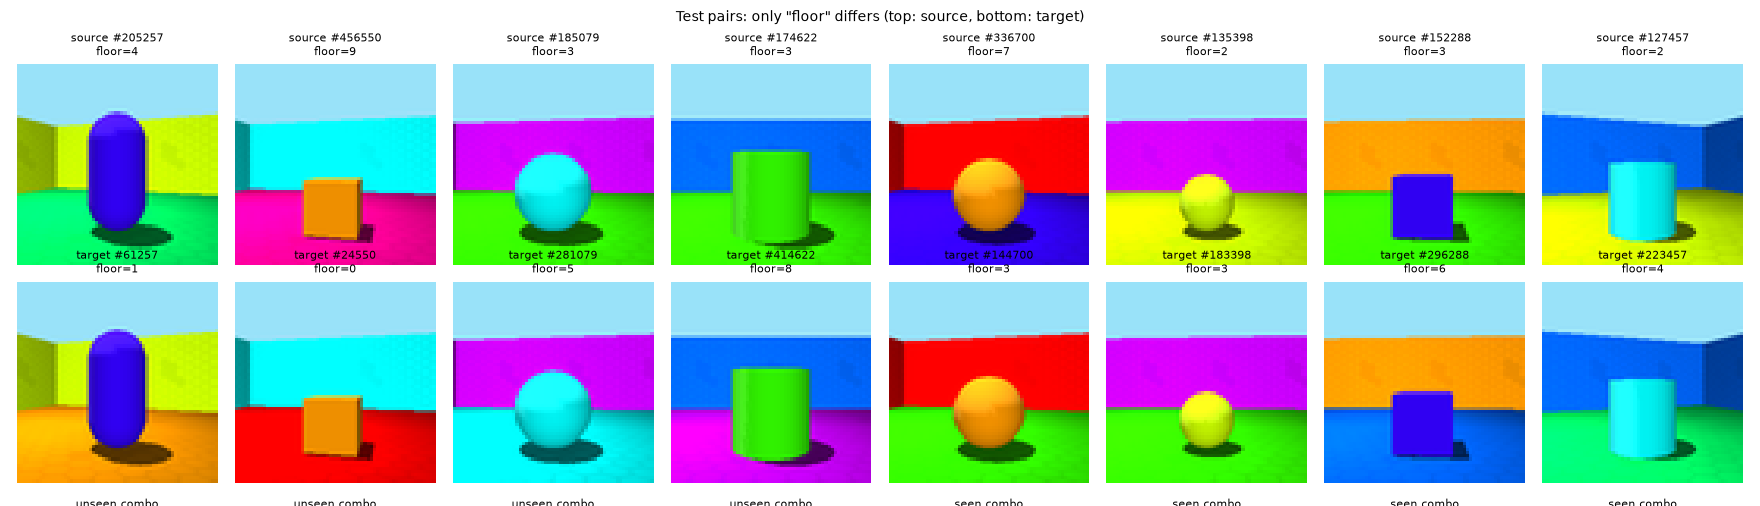
\includegraphics[width=\textwidth]{figures/montage_shapes3d.png}\\[2pt]
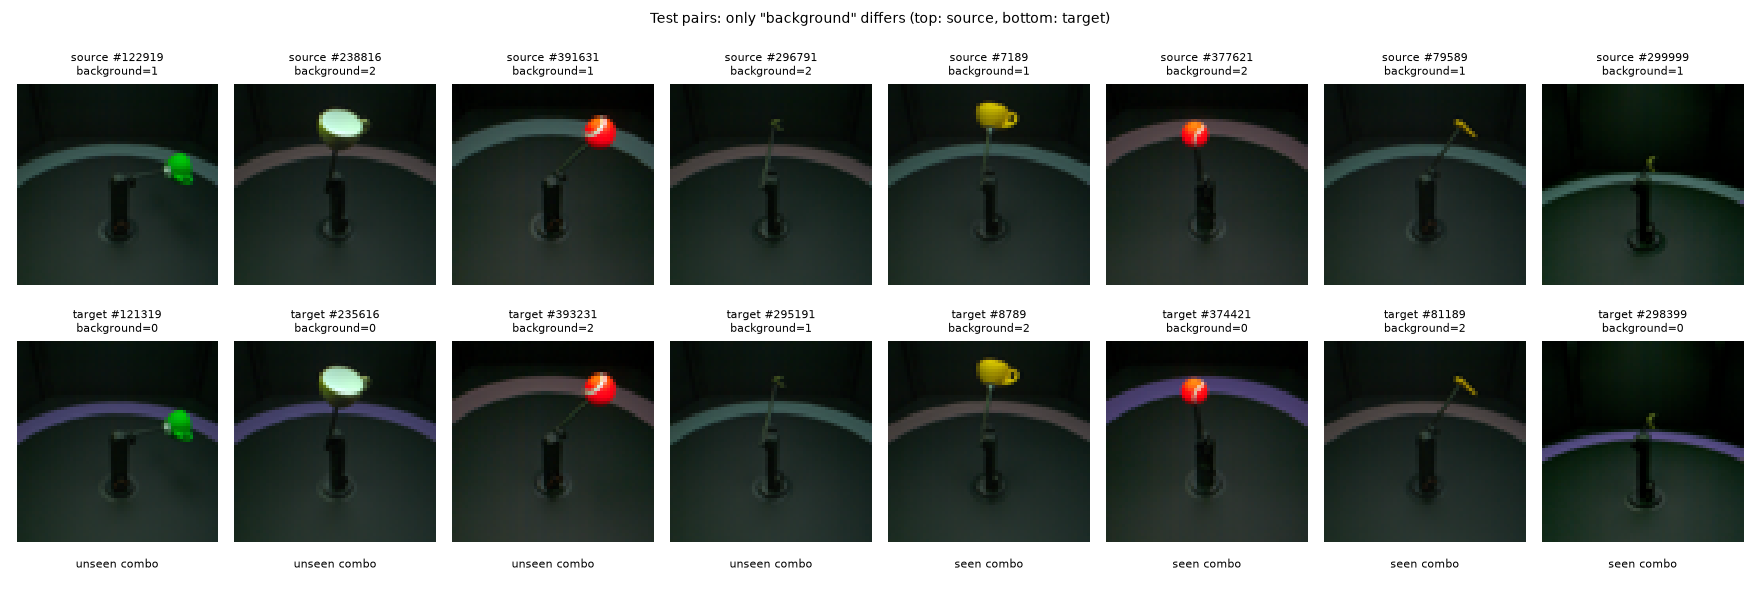
\includegraphics[width=\textwidth]{figures/montage_mpi3d.png}
\caption{Representative test pairs (top row source, bottom row target). Shapes3D: only the floor colour changes.
MPI3D (real photos of a robot arm): only the coloured background ring changes.}
\label{fig:montage}
\end{figure}

\subsection{Split before fitting or selecting operators}

\begin{table}[H]
\centering\small
\begin{tabularx}{\textwidth}{p{5.6cm}p{1.4cm}L}
\toprule
Plan item & Status & What was done / change made \\
\midrule
Group by all unchanged factors (contexts) & \done & Context $=$ all raw factors except the edited one; contexts split 60/20/20 \emph{before} pairs are drawn. \\
Disjoint operator-train / val / test groups & \done & Asserted on contexts. \\
No endpoint crosses splits; check hashes and IDs & \done & Asserted on IDs and on SHA-1 of the stored image bytes (no duplicate image bytes exist in either dataset). \\
Unseen-combination evaluation, independent of held-out contexts & \done & Some (edit value, \code{shape}) conjunctions never appear at either endpoint of a train/val pair; every value and every shape still appears in training. Rule: $(v + 3s) \bmod 10 < 2$ (Shapes3D), $(v+s)\bmod 3<1$ (MPI3D). \\
Did test endpoints appear in base-model training? & \done & Yes, all images did. The claim is \textbf{scoped to operator generalization}; a separate stratum keeps pairs whose two images were only in the base model's eval cache. \\
Splits fixed across seeds and baselines & \done & One pair manifest per dataset; its hash is checked at evaluation. \\
Normalization, probes, hyperparameters on permitted folds only & \partly & Normalization, readers, calibration and checkpoint selection use train/val only. One exception during development is disclosed in Sec.~\ref{sec:deviation}. \\
\midrule
\multicolumn{3}{p{0.95\textwidth}}{\textbf{Done when} automated assertions establish validity and disjointness: \done{} (\code{validate_pairs}, 6 unit tests).} \\
\bottomrule
\end{tabularx}
\caption{Splits. The row-random cache splitter was not used.}
\end{table}

\begin{table}[H]
\centering\small
\begin{tabular}{llrrrrr}
\toprule
Dataset & Split & Contexts & Pairs & Endpoint images & Unseen-combination pairs & Base-heldout pairs \\
\midrule
Shapes3D & train & 28,800 & 172,800 & 193,418 & 0 & 6,990 \\
Shapes3D & val & 9,600 & 57,600 & 64,329 & 0 & 2,274 \\
Shapes3D & test & 9,600 & 57,600 & 71,789 & 11,424 & 2,325 \\
\midrule
MPI3D & train & 92,160 & 184,320 & 184,320 & 0 & 7,134 \\
MPI3D & val & 30,720 & 61,440 & 61,440 & 0 & 2,504 \\
MPI3D & test & 30,720 & 61,440 & 86,048 & 20,463 & 2,524 \\


\bottomrule
\end{tabular}
\caption{Pair manifests (6 pairs per context for Shapes3D, 2 for MPI3D). ``Base-heldout'': both images only in the
base model's evaluation cache.}
\end{table}

\subsection{Connect the experiment to native models}

\begin{table}[H]
\centering\small
\begin{tabularx}{\textwidth}{p{5.6cm}p{1.4cm}L}
\toprule
Plan item & Status & What was done / change made \\
\midrule
Adapter: rebuild, \code{eval()}, freeze, expose operations & \done & \code{load_student} (strict state dict, eval mode, \code{requires_grad=False}); exposes \code{encode}, \code{concept_readout}, \code{predict_from_concepts}, \code{intervene}. \\
Same backbone/preprocessing for both endpoints & \done & Both endpoints read from the same full feature cache (verified equal to the train/eval caches row by row). \\
Cache latents with IDs and checkpoint hashes & \done & \code{cached_latents}: refuses a cache made from a different checkpoint or ID file (SHA-256). \\
Validate readout units & \done & Units are BCE logits; logit-unit interventions verified to decode to the target. This check revealed that the readout is poorly calibrated (Sec.~\ref{sec:gate}); calibrated decoding was added. \\
Latent coordinates vs supervised readouts (CEM) & \done & Native intervention acts through the readout; donor substitution uses the full concept block; learned operators act on the full latent. \\
Adapter reproduces the ordinary forward pass & \done & Asserted in every run (accuracy within $1/n$) and in unit tests (exact equality). \\
\bottomrule
\end{tabularx}
\caption{Native adapter (\code{native_adapter.py}); the NumPy toy models remain software controls.}
\end{table}

\subsection{Minimum operator comparison}

\begin{table}[H]
\centering\small
\begin{tabularx}{\textwidth}{p{5.6cm}p{1.4cm}L}
\toprule
Plan item & Status & What was done / change made \\
\midrule
All arms (identity, native, affine, MLP, real image, donor) & \done & Seven arms: native in two unit conventions (Sec.~\ref{sec:intervention}). \\
Affine and MLP in PyTorch, same pair/action schema & \done & \code{torch_operators.py}; action $=$ one-hot target level. \\
Freeze encoder and readers; optimise only the operator & \done & Only operator parameters are passed to the optimiser. \\
Paired latent reconstruction, selection on validation & \done & MSE in standardized latent space; Adam, lr $10^{-3}$, batch 2048, 10{,}000 steps; checkpoint with lowest validation-pair MSE. \\
Extra preservation/readout loss as separate ablation & \notdone & Not run; operators use reconstruction only (so no extra supervision explains any gain). \\
No target-image access at inference & \done & Operator signature is $(x, a)$; tested. \\
Report parameters, pairs, budget, selection rule & \done & Table~\ref{tab:operators}; recorded in each \code{train_config.json}. \\
\bottomrule
\end{tabularx}
\caption{Operators (\code{torch_operators.py}, \code{train_native.py}). 3 operator seeds per checkpoint.}
\end{table}

\begin{table}[H]
\centering\small
\begin{tabular}{lrrrrllr}
\toprule
Run & $d$ & Affine params & MLP params & Train pairs & Affine sel.\ step & MLP sel.\ step & Reader val.\ acc. \\
\midrule
Shapes3D CBM s0 & 16 & 432 & 76,816 & 172,800 & 7200/5800/9000 & 10000/9600/9600 & 0.874 \\
Shapes3D CBM s12 & 16 & 432 & 76,816 & 172,800 & 9200/5800/7200 & 9200/10000/10000 & 0.881 \\
Shapes3D CEM s0 & 32 & 1,376 & 85,024 & 172,800 & 7200/6400/9000 & 10000/9800/10000 & 0.951 \\
Shapes3D CEM s12 & 32 & 1,376 & 85,024 & 172,800 & 5000/9400/9800 & 10000/9800/10000 & 0.952 \\
MPI3D CBM s12 & 20 & 480 & 77,076 & 184,320 & 10000/10000/9000 & 9600/10000/9800 & 0.800 \\
MPI3D CEM s12 & 40 & 1,760 & 87,336 & 184,320 & 9600/8800/7800 & 9800/9200/10000 & 0.854 \\

\bottomrule
\end{tabular}
\caption{Operator size, data and selected step for seeds 0/1/2 (budget 10{,}000 steps), and mean validation accuracy
of the readers over all factors.}
\label{tab:operators}
\end{table}

\subsection{Evaluate behaviour, not only latent distance}

\begin{table}[H]
\centering\small
\begin{tabularx}{\textwidth}{p{5.6cm}p{1.4cm}L}
\toprule
Plan item & Status & What was done / change made \\
\midrule
Target success (tolerance for continuous factors) & \partly & Edited factor read as the requested level. All factors are treated as discrete levels; no continuous tolerance was predeclared, so none is applied. \\
Preservation, and retention conditional on initial correctness & \done & All other raw factors read correctly; conditional retention among pairs whose source was read correctly. Per-factor preservation also reported. \\
Task outcome, changed- vs invariant-label & \partly & Only the invariant-label case exists in this schema. \\
Joint success & \done & Target $\wedge$ preservation $\wedge$ task correct. \\
Reference quality & \done & Reader accuracy on source and target images, task accuracy (Table~\ref{tab:readers}). \\
Seen vs unseen combinations, held-out contexts & \done & All test pairs are in held-out contexts; stratified seen/unseen and base-heldout. \\
Latent discrepancy as secondary & \done & Standardized latent MSE, reported but not used for conclusions. \\
Per-example exports & \done & \code{per_pair.csv.gz} (IDs, split, context, seed, checkpoint, action, ground truth, readings, metrics) and \code{readouts_logits.npz}. \\
Paired resampling of context groups; independent seeds & \done & Context bootstrap (2000 resamples) of paired differences, per operator seed; 3 operator seeds; 2 model seeds on Shapes3D. \\
Main and qualitative figures & \done & Figures~\ref{fig:main} and \ref{fig:qual}. \\
\bottomrule
\end{tabularx}
\caption{Evaluation (\code{evaluate_native.py}, run once per checkpoint; \code{summarize_native.py}).}
\end{table}

\subsection{Decision gate, after-gate items and code}

The four gate checks are answered in Section~\ref{sec:gate}. After-gate items:

\begin{table}[H]
\centering\small
\begin{tabularx}{\textwidth}{p{5.6cm}p{1.6cm}L}
\toprule
Item & Status & Comment \\
\midrule
Composed edits & \na & Gate not passed. \\
Second architecture (CEM) & \done & CEM checkpoints existed, so CBM and CEM were evaluated from the start. \\
Natural-image setting & \na & CUB has no edited-image pairs; would need verified generated edits. \\
Related-work audit & \notdone & --- \\
Reproducible table, figures, configurations, commands & \done & This document, \code{README.md}, \code{summary/}, \code{train_config.json} with source hashes. \\
\bottomrule
\end{tabularx}
\end{table}

All proposed files were created: \code{inventory.py}, \code{build_pairs.py}, \code{native_adapter.py},
\code{torch_operators.py}, \code{train_native.py}, \code{evaluate_native.py}, \code{tests/test_semantic_edit_pairs.py},
\code{tests/test_semantic_edit_adapter.py}, plus \code{summarize_native.py} (tables, figures, gate evidence). Shared
models, extraction and cache utilities were reused in place.

%==============================================================================
\section{Held-out readers: why and how}
\label{sec:readers}
%==============================================================================

The native intervention sets the model's own concept readout \emph{by construction}; judging it with that readout
would be circular. The plan allows held-out readers ``only if needed''; they were needed.

\begin{itemize}
\item One MLP (two hidden layers of 256 units) with one softmax head per raw factor, including the factors the model
  was never supervised on (object colour, shape).
\item Input: standardized latent state. Trained on 150{,}000 \emph{original, unedited} images from operator-training
  contexts (8{,}000 steps), selected on validation-context images by mean accuracy. Never trained on edited states or
  test images.
\item Readers may see images of held-out (value, shape) combinations from training contexts: they are measuring
  instruments, and only the edit operators must never be fitted on a held-out combination.
\end{itemize}

Because readers are imperfect, the \textbf{real edited image is the practical ceiling} of every metric; methods
should be compared with it rather than with $1$.

\begin{table}[H]
\centering\small
\begin{tabular}{lrrrrrrr}
\toprule
Run & floor & wall & object & scale & shape & orientation & task \\
\midrule
Shapes3D CBM s0 & 0.839 & 0.787 & 0.998 & 0.868 & 1.000 & 0.761 & 0.986 \\
Shapes3D CBM s12 & 0.853 & 0.802 & 0.998 & 0.857 & 1.000 & 0.773 & 0.977 \\
Shapes3D CEM s0 & 0.947 & 0.933 & 0.998 & 0.896 & 1.000 & 0.936 & 0.994 \\
Shapes3D CEM s12 & 0.955 & 0.924 & 0.998 & 0.901 & 1.000 & 0.938 & 0.985 \\

\bottomrule
\end{tabular}

\smallskip
\begin{tabular}{lrrrrrrrr}
\toprule
Run & color & shape & size & height & background & dof1 & dof2 & task \\
\midrule
MPI3D CBM s12 & 1.000 & 1.000 & 0.995 & 1.000 & 1.000 & 0.279 & 0.331 & 1.000 \\
MPI3D CEM s12 & 1.000 & 1.000 & 0.995 & 1.000 & 1.000 & 0.435 & 0.552 & 1.000 \\

\bottomrule
\end{tabular}
\caption{Reader accuracy per raw factor on the real edited (target) test images, and task accuracy on source
images. MPI3D arm positions (\code{dof1}, \code{dof2}, 40 levels each) are read poorly even on real images.}
\label{tab:readers}
\end{table}

%==============================================================================
\section{Results}
%==============================================================================

Metrics (all on test pairs, read by the held-out readers unless stated):
\textbf{target success} (edited factor read as requested);
\textbf{preservation} (all other raw factors read correctly);
\textbf{conditional retention} (preservation among pairs whose source was read correctly);
\textbf{task} (task head correct; the label is invariant);
\textbf{joint} (all three);
\textbf{native target} (the model's own readout decodes the requested level, calibrated decoding).
Learned operators: mean $\pm$ s.d.\ over 3 operator seeds. $^\dagger$: uses the target image (reference).

\begin{table}[H]
\centering\small
\begin{tabular}{lrrrrrr}
\toprule
Method & \shortstack{Shapes3D\\CBM s0} & \shortstack{Shapes3D\\CBM s12} & \shortstack{Shapes3D\\CEM s0} & \shortstack{Shapes3D\\CEM s12} & \shortstack{MPI3D\\CBM s12} & \shortstack{MPI3D\\CEM s12}
 \\
\midrule
Identity & 0.007 & 0.007 & 0.003 & 0.003 & 0.000 & 0.000 \\
\midrule
Native (logit) & 0.042 & 0.013 & 0.079 & 0.052 & 0.071 & 0.125 \\
Native (calibrated) & 0.103 & 0.050 & 0.100 & 0.088 & 0.072 & 0.130 \\
\midrule
Affine & 0.208\,{\scriptsize$\pm$0.001} & 0.199\,{\scriptsize$\pm$0.001} & 0.388\,{\scriptsize$\pm$0.002} & 0.376\,{\scriptsize$\pm$0.000} & 0.056\,{\scriptsize$\pm$0.000} & 0.137\,{\scriptsize$\pm$0.000} \\
MLP & 0.237\,{\scriptsize$\pm$0.001} & 0.253\,{\scriptsize$\pm$0.009} & 0.434\,{\scriptsize$\pm$0.009} & 0.435\,{\scriptsize$\pm$0.007} & 0.040\,{\scriptsize$\pm$0.002} & 0.125\,{\scriptsize$\pm$0.001} \\
\midrule
Donor block$^\dagger$ & 0.154 & 0.143 & 0.206 & 0.186 & 0.065 & 0.090 \\
Real edited image$^\dagger$ & 0.437 & 0.444 & 0.737 & 0.731 & 0.088 & 0.234 \\

\bottomrule
\end{tabular}
\caption{\textbf{Main result.} Joint success on unseen-combination test pairs (identical pairs for all methods).}
\label{tab:main}
\end{table}

\begin{figure}[H]
\centering
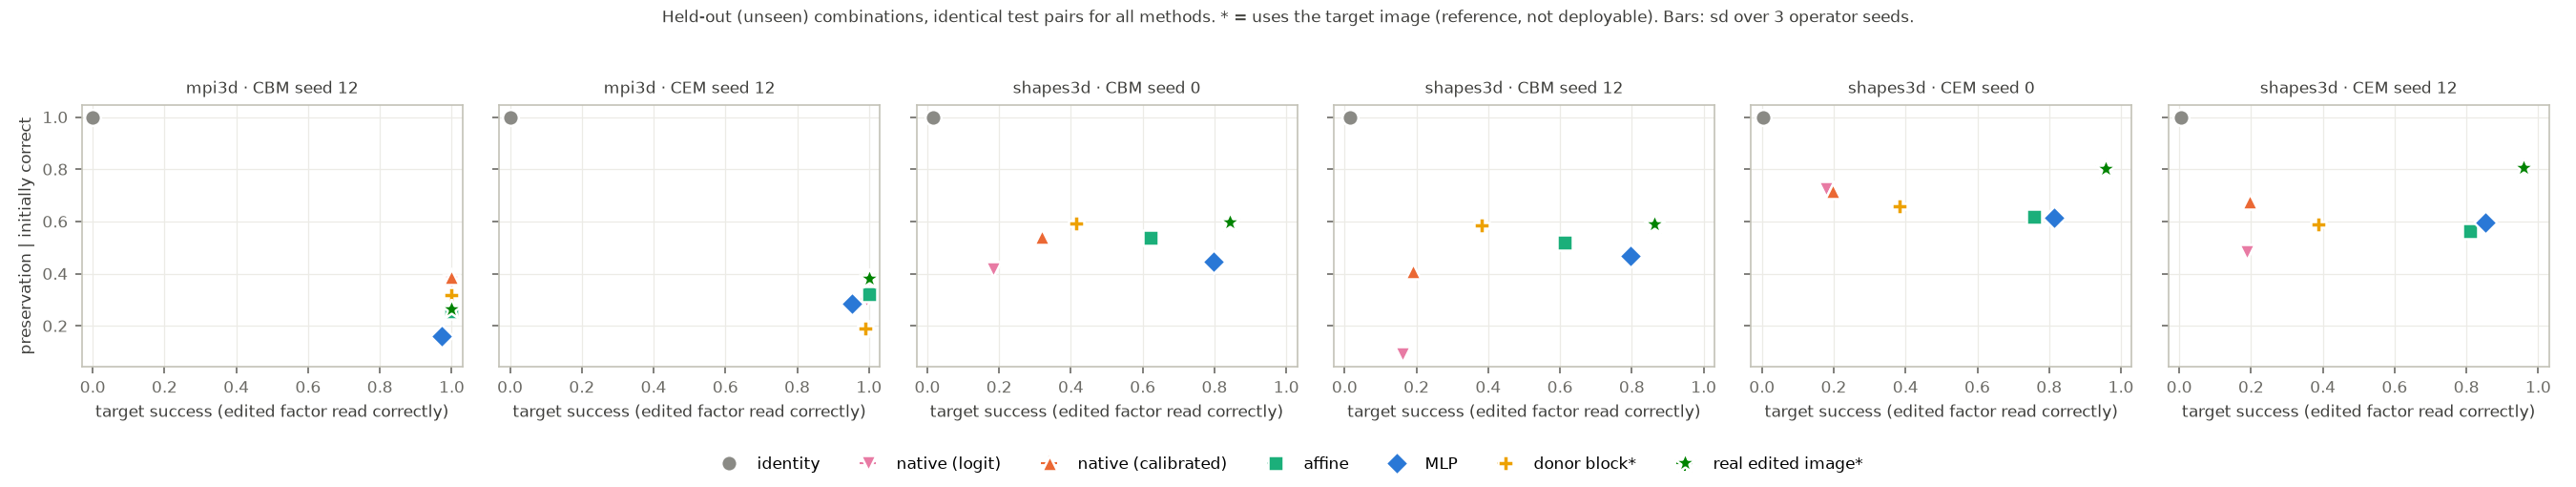
\includegraphics[width=\textwidth]{figures/target_vs_preservation.png}
\caption{Target success versus conditional retention on unseen combinations, identical test pairs for all methods.
Bars: s.d.\ over operator seeds. The ideal point is the top right; the real edited image ($\star$) is the
attainable reference.}
\label{fig:main}
\end{figure}

\begin{table}[H]
\centering\footnotesize
\begin{tabular}{lrrrrrrr}
\toprule
Method & Target & Cond.\ retention & Preservation & Task & Joint & Native target & Latent MSE \\
\midrule
\multicolumn{8}{l}{\textbf{Shapes3D CBM s0}} \\
\quad Identity & 0.015 & 1.000 & 0.528 & 0.986 & 0.007 & 0.060 & 0.397 \\
\quad Native (logit) & 0.184 & 0.418 & 0.277 & 0.986 & 0.042 & 0.125 & 0.228 \\
\quad Native (calibrated) & 0.320 & 0.541 & 0.349 & 0.986 & 0.103 & 1.000 & 0.169 \\
\quad Affine & 0.623\,{\scriptsize$\pm$0.001} & 0.538\,{\scriptsize$\pm$0.001} & 0.353\,{\scriptsize$\pm$0.001} & 0.950\,{\scriptsize$\pm$0.001} & 0.208\,{\scriptsize$\pm$0.001} & 0.510\,{\scriptsize$\pm$0.012} & 0.134\,{\scriptsize$\pm$0.000} \\
\quad MLP & 0.798\,{\scriptsize$\pm$0.006} & 0.446\,{\scriptsize$\pm$0.002} & 0.305\,{\scriptsize$\pm$0.002} & 0.977\,{\scriptsize$\pm$0.002} & 0.237\,{\scriptsize$\pm$0.001} & 0.452\,{\scriptsize$\pm$0.028} & 0.109\,{\scriptsize$\pm$0.003} \\
\quad Donor block$^\dagger$ & 0.415 & 0.593 & 0.395 & 0.979 & 0.154 & 0.373 & 0.113 \\
\quad Real edited image$^\dagger$ & 0.843 & 0.596 & 0.517 & 0.986 & 0.437 & 0.373 & 0.000 \\
\midrule
\multicolumn{8}{l}{\textbf{Shapes3D CBM s12}} \\
\quad Identity & 0.015 & 1.000 & 0.541 & 0.979 & 0.007 & 0.055 & 0.379 \\
\quad Native (logit) & 0.161 & 0.089 & 0.068 & 0.980 & 0.013 & 0.125 & 0.441 \\
\quad Native (calibrated) & 0.192 & 0.411 & 0.281 & 0.975 & 0.050 & 1.000 & 0.183 \\
\quad Affine & 0.613\,{\scriptsize$\pm$0.001} & 0.519\,{\scriptsize$\pm$0.001} & 0.349\,{\scriptsize$\pm$0.000} & 0.944\,{\scriptsize$\pm$0.001} & 0.199\,{\scriptsize$\pm$0.001} & 0.347\,{\scriptsize$\pm$0.002} & 0.130\,{\scriptsize$\pm$0.000} \\
\quad MLP & 0.795\,{\scriptsize$\pm$0.011} & 0.467\,{\scriptsize$\pm$0.017} & 0.330\,{\scriptsize$\pm$0.011} & 0.962\,{\scriptsize$\pm$0.001} & 0.253\,{\scriptsize$\pm$0.009} & 0.325\,{\scriptsize$\pm$0.010} & 0.098\,{\scriptsize$\pm$0.001} \\
\quad Donor block$^\dagger$ & 0.381 & 0.586 & 0.400 & 0.960 & 0.143 & 0.262 & 0.121 \\
\quad Real edited image$^\dagger$ & 0.862 & 0.589 & 0.523 & 0.970 & 0.444 & 0.262 & 0.000 \\
\midrule
\multicolumn{8}{l}{\textbf{Shapes3D CEM s0}} \\
\quad Identity & 0.004 & 1.000 & 0.783 & 0.995 & 0.003 & 0.076 & 0.456 \\
\quad Native (logit) & 0.179 & 0.725 & 0.605 & 0.995 & 0.079 & 0.372 & 0.374 \\
\quad Native (calibrated) & 0.198 & 0.716 & 0.600 & 0.995 & 0.100 & 1.000 & 0.358 \\
\quad Affine & 0.759\,{\scriptsize$\pm$0.003} & 0.618\,{\scriptsize$\pm$0.001} & 0.534\,{\scriptsize$\pm$0.000} & 0.937\,{\scriptsize$\pm$0.001} & 0.388\,{\scriptsize$\pm$0.002} & 0.330\,{\scriptsize$\pm$0.005} & 0.252\,{\scriptsize$\pm$0.000} \\
\quad MLP & 0.814\,{\scriptsize$\pm$0.025} & 0.615\,{\scriptsize$\pm$0.006} & 0.538\,{\scriptsize$\pm$0.004} & 0.980\,{\scriptsize$\pm$0.003} & 0.434\,{\scriptsize$\pm$0.009} & 0.312\,{\scriptsize$\pm$0.027} & 0.194\,{\scriptsize$\pm$0.002} \\
\quad Donor block$^\dagger$ & 0.383 & 0.657 & 0.569 & 0.987 & 0.206 & 0.279 & 0.251 \\
\quad Real edited image$^\dagger$ & 0.957 & 0.802 & 0.771 & 0.994 & 0.737 & 0.279 & 0.000 \\
\midrule
\multicolumn{8}{l}{\textbf{Shapes3D CEM s12}} \\
\quad Identity & 0.004 & 1.000 & 0.783 & 0.986 & 0.003 & 0.066 & 0.494 \\
\quad Native (logit) & 0.188 & 0.483 & 0.417 & 0.985 & 0.052 & 0.372 & 0.449 \\
\quad Native (calibrated) & 0.197 & 0.676 & 0.572 & 0.984 & 0.088 & 1.000 & 0.399 \\
\quad Affine & 0.810\,{\scriptsize$\pm$0.001} & 0.564\,{\scriptsize$\pm$0.001} & 0.486\,{\scriptsize$\pm$0.001} & 0.933\,{\scriptsize$\pm$0.001} & 0.376\,{\scriptsize$\pm$0.000} & 0.297\,{\scriptsize$\pm$0.002} & 0.276\,{\scriptsize$\pm$0.000} \\
\quad MLP & 0.853\,{\scriptsize$\pm$0.020} & 0.594\,{\scriptsize$\pm$0.004} & 0.520\,{\scriptsize$\pm$0.003} & 0.971\,{\scriptsize$\pm$0.001} & 0.435\,{\scriptsize$\pm$0.007} & 0.247\,{\scriptsize$\pm$0.013} & 0.216\,{\scriptsize$\pm$0.005} \\
\quad Donor block$^\dagger$ & 0.388 & 0.590 & 0.513 & 0.977 & 0.186 & 0.247 & 0.293 \\
\quad Real edited image$^\dagger$ & 0.960 & 0.805 & 0.771 & 0.984 & 0.731 & 0.247 & 0.000 \\
\midrule
\multicolumn{8}{l}{\textbf{MPI3D CBM s12}} \\
\quad Identity & 0.000 & 1.000 & 0.091 & 1.000 & 0.000 & 0.000 & 0.374 \\
\quad Native (logit) & 1.000 & 0.364 & 0.071 & 1.000 & 0.071 & 1.000 & 0.053 \\
\quad Native (calibrated) & 1.000 & 0.386 & 0.072 & 1.000 & 0.072 & 1.000 & 0.051 \\
\quad Affine & 1.000\,{\scriptsize$\pm$0.000} & 0.257\,{\scriptsize$\pm$0.003} & 0.056\,{\scriptsize$\pm$0.000} & 1.000\,{\scriptsize$\pm$0.000} & 0.056\,{\scriptsize$\pm$0.000} & 1.000\,{\scriptsize$\pm$0.000} & 0.058\,{\scriptsize$\pm$0.000} \\
\quad MLP & 0.973\,{\scriptsize$\pm$0.005} & 0.159\,{\scriptsize$\pm$0.003} & 0.042\,{\scriptsize$\pm$0.002} & 0.996\,{\scriptsize$\pm$0.000} & 0.040\,{\scriptsize$\pm$0.002} & 0.962\,{\scriptsize$\pm$0.014} & 0.093\,{\scriptsize$\pm$0.002} \\
\quad Donor block$^\dagger$ & 0.999 & 0.317 & 0.065 & 1.000 & 0.065 & 0.999 & 0.044 \\
\quad Real edited image$^\dagger$ & 1.000 & 0.263 & 0.088 & 1.000 & 0.088 & 0.999 & 0.000 \\
\midrule
\multicolumn{8}{l}{\textbf{MPI3D CEM s12}} \\
\quad Identity & 0.000 & 1.000 & 0.230 & 1.000 & 0.000 & 0.000 & 0.306 \\
\quad Native (logit) & 0.991 & 0.300 & 0.126 & 1.000 & 0.125 & 1.000 & 0.146 \\
\quad Native (calibrated) & 0.990 & 0.324 & 0.132 & 1.000 & 0.130 & 1.000 & 0.145 \\
\quad Affine & 1.000\,{\scriptsize$\pm$0.000} & 0.323\,{\scriptsize$\pm$0.000} & 0.137\,{\scriptsize$\pm$0.000} & 1.000\,{\scriptsize$\pm$0.000} & 0.137\,{\scriptsize$\pm$0.000} & 1.000\,{\scriptsize$\pm$0.000} & 0.111\,{\scriptsize$\pm$0.000} \\
\quad MLP & 0.953\,{\scriptsize$\pm$0.005} & 0.284\,{\scriptsize$\pm$0.008} & 0.131\,{\scriptsize$\pm$0.003} & 0.997\,{\scriptsize$\pm$0.000} & 0.125\,{\scriptsize$\pm$0.001} & 0.881\,{\scriptsize$\pm$0.011} & 0.126\,{\scriptsize$\pm$0.003} \\
\quad Donor block$^\dagger$ & 0.990 & 0.191 & 0.091 & 1.000 & 0.090 & 0.999 & 0.118 \\
\quad Real edited image$^\dagger$ & 1.000 & 0.380 & 0.234 & 1.000 & 0.234 & 0.999 & 0.000 \\

\bottomrule
\end{tabular}
\caption{All metrics on unseen-combination test pairs.}
\label{tab:detail}
\end{table}

\begin{figure}[H]
\centering
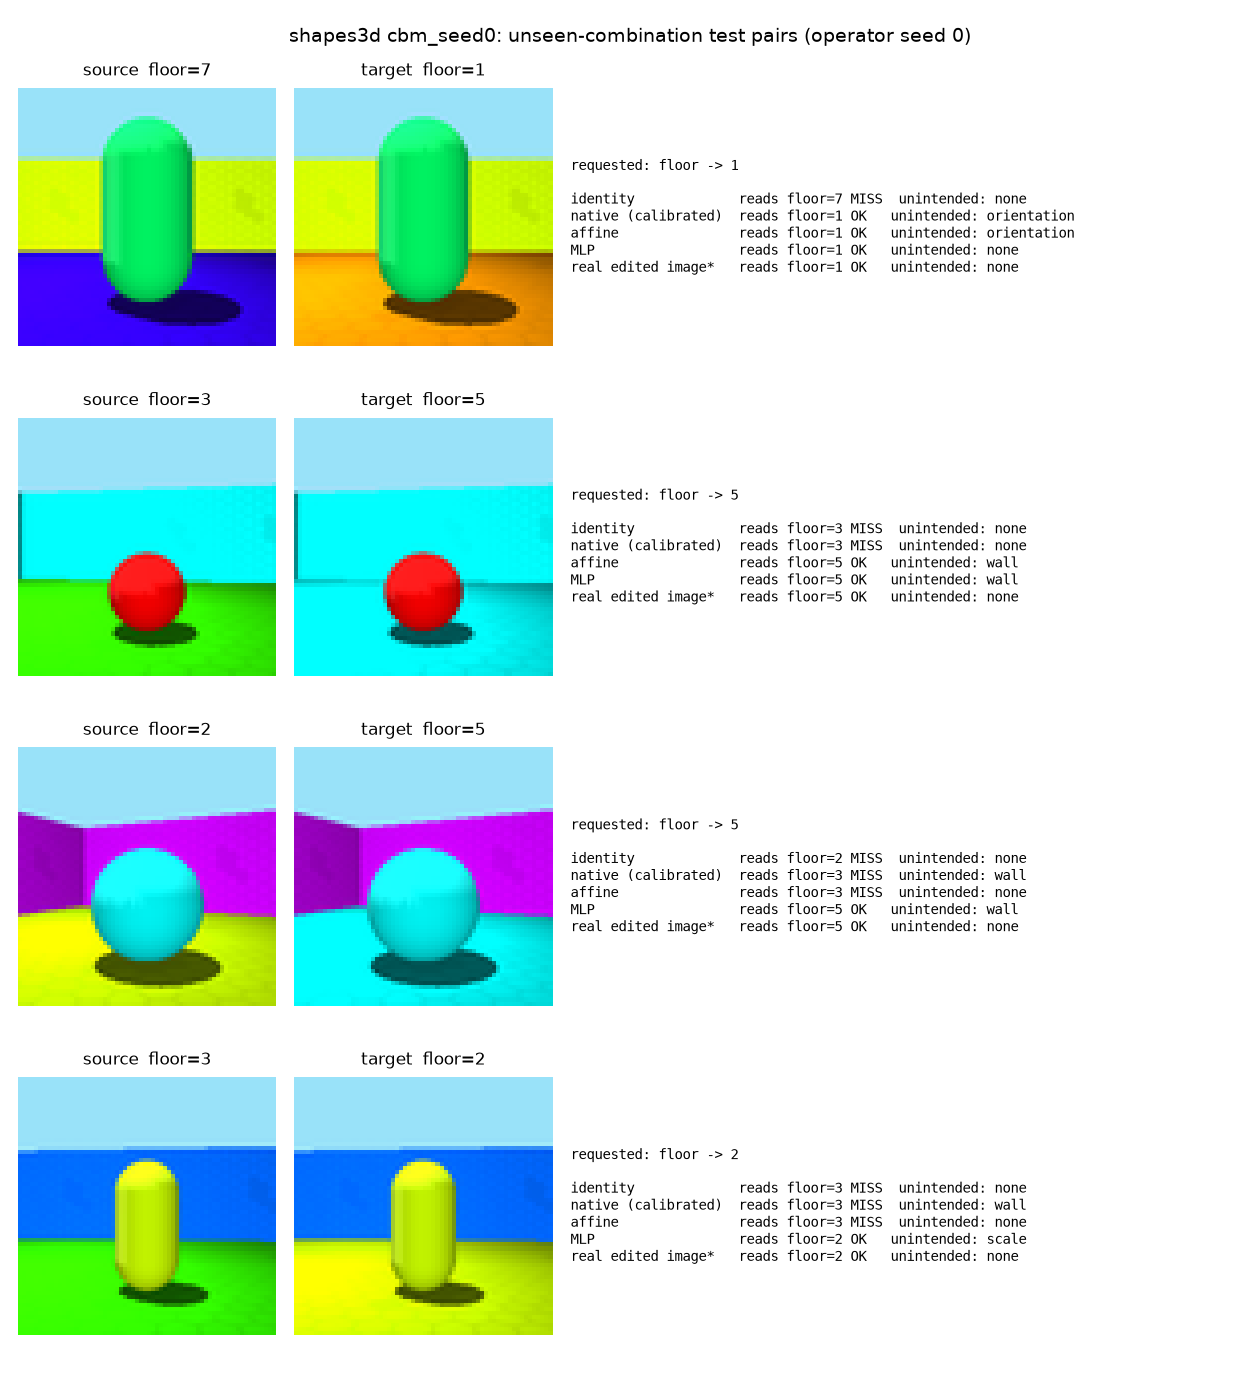
\includegraphics[width=0.92\textwidth]{figures/qualitative_shapes3d.png}
\caption{Qualitative examples (Shapes3D CBM seed 0, unseen combinations, operator seed 0): what each method's edited
state reads as, for the requested factor and for unintended changes.}
\label{fig:qual}
\end{figure}

%==============================================================================
\section{Decision gate and interpretation}
\label{sec:gate}
%==============================================================================

\subsection{Gate 1: is the native failure a unit error or poor perception?}

\begin{table}[H]
\centering\small
\begin{tabular}{lrrrrrr}
\toprule
& \multicolumn{2}{c}{Own readout decodes edit factor} & Readers on & \multicolumn{3}{c}{Native intervention, unseen pairs} \\
\cmidrule(lr){2-3}\cmidrule(lr){5-7}
Run & sigmoid & calibrated & real images & own readout & readers (cal.) & readers (logit) \\
\midrule
Shapes3D CBM s0 & 0.186 & 0.422 & 0.839 & 1.000 & 0.320 & 0.184 \\
Shapes3D CBM s12 & 0.117 & 0.345 & 0.853 & 1.000 & 0.192 & 0.161 \\
Shapes3D CEM s0 & 0.302 & 0.332 & 0.947 & 1.000 & 0.198 & 0.179 \\
Shapes3D CEM s12 & 0.224 & 0.329 & 0.955 & 1.000 & 0.197 & 0.188 \\
MPI3D CBM s12 & 0.982 & 0.996 & 1.000 & 1.000 & 1.000 & 1.000 \\
MPI3D CEM s12 & 0.982 & 0.996 & 1.000 & 1.000 & 0.990 & 0.991 \\

\bottomrule
\end{tabular}
\caption{Native intervention diagnostics. ``Own readout'': the model's concept readout decodes the requested level
after intervention.}
\label{tab:native}
\end{table}

\begin{itemize}
\item \textbf{Not a unit error.} With calibrated values, the model's own readout reports the requested floor for
  $100\%$ of pairs, yet the independent readers see it in only $19$--$32\%$. The logit convention is no better.
\item \textbf{Not poor perception of the latent.} The latent encodes the floor: readers find it in $84$--$95\%$ of
  real images.
\item \textbf{But the concept readout is weak.} On Shapes3D, the model's own readout decodes the floor level for only
  $12$--$30\%$ of images (sigmoid) or $33$--$42\%$ (calibrated). The floor information is mostly stored outside the
  readout direction, in the free coordinates, which the native intervention never touches.
\item On MPI3D the readout is accurate ($98$--$99.6\%$) and the native intervention works.
\end{itemize}

\subsection{Gates 2--4: nonlinear versus affine, preservation, seeds}

\begin{table}[H]
\centering\footnotesize
\begin{tabular}{llll}
\toprule
Run & MLP $-$ affine & MLP $-$ native (cal.) & Affine $-$ native (cal.) \\
\midrule
Shapes3D CBM s0 & +0.027 / +0.030 / +0.030 {\scriptsize[+0.016, +0.041]} & +0.134 / +0.136 / +0.137 {\scriptsize[+0.124, +0.148]} & +0.107 / +0.106 / +0.108 {\scriptsize[+0.097, +0.116]} \\
Shapes3D CBM s12 & +0.058 / +0.060 / +0.041 {\scriptsize[+0.031, +0.071]} & +0.207 / +0.209 / +0.191 {\scriptsize[+0.181, +0.219]} & +0.148 / +0.148 / +0.149 {\scriptsize[+0.140, +0.158]} \\
Shapes3D CEM s0 & +0.042 / +0.032 / +0.048 {\scriptsize[+0.019, +0.060]} & +0.335 / +0.322 / +0.343 {\scriptsize[+0.311, +0.354]} & +0.293 / +0.291 / +0.295 {\scriptsize[+0.280, +0.306]} \\
Shapes3D CEM s12 & +0.057 / +0.061 / +0.043 {\scriptsize[+0.031, +0.073]} & +0.347 / +0.350 / +0.333 {\scriptsize[+0.322, +0.361]} & +0.291 / +0.289 / +0.290 {\scriptsize[+0.278, +0.302]} \\
MPI3D CBM s12 & -0.015 / -0.018 / -0.014 {\scriptsize[-0.022, -0.010]} & -0.030 / -0.034 / -0.030 {\scriptsize[-0.038, -0.026]} & -0.016 / -0.016 / -0.016 {\scriptsize[-0.020, -0.012]} \\
MPI3D CEM s12 & -0.011 / -0.009 / -0.011 {\scriptsize[-0.017, -0.003]} & -0.005 / -0.003 / -0.005 {\scriptsize[-0.011, +0.004]} & +0.006 / +0.007 / +0.006 {\scriptsize[+0.000, +0.013]} \\

\bottomrule
\end{tabular}
\caption{Paired differences in joint success on unseen combinations, for operator seeds 0/1/2, with the widest
95\% context-bootstrap interval over the three seeds.}
\label{tab:boot}
\end{table}

\begin{table}[H]
\centering\footnotesize
\begin{tabular}{lrrrrrrrr}
\toprule
& \multicolumn{3}{c}{Affine joint} & \multicolumn{3}{c}{MLP joint} & Cond.\ retention & MLP / \\
\cmidrule(lr){2-4}\cmidrule(lr){5-7}
Run & seen & unseen & $\Delta$ & seen & unseen & $\Delta$ & MLP $-$ affine & reference \\
\midrule
Shapes3D CBM s0 & 0.218 & 0.208 & -0.011 & 0.338 & 0.237 & -0.101 & -0.093 & 0.54 \\
Shapes3D CBM s12 & 0.203 & 0.199 & -0.004 & 0.353 & 0.253 & -0.100 & -0.052 & 0.57 \\
Shapes3D CEM s0 & 0.396 & 0.388 & -0.008 & 0.585 & 0.434 & -0.151 & -0.003 & 0.59 \\
Shapes3D CEM s12 & 0.403 & 0.376 & -0.027 & 0.566 & 0.435 & -0.131 & +0.031 & 0.59 \\
MPI3D CBM s12 & 0.073 & 0.056 & -0.018 & 0.079 & 0.040 & -0.039 & -0.098 & 0.46 \\
MPI3D CEM s12 & 0.169 & 0.137 & -0.032 & 0.210 & 0.125 & -0.085 & -0.039 & 0.54 \\

\bottomrule
\end{tabular}
\caption{Seen versus unseen combinations, preservation difference, and MLP joint success as a fraction of the
real-image reference (unseen).}
\label{tab:seen}
\end{table}

\begin{itemize}
\item \textbf{Gate 2 (MLP vs affine on held-out combinations).} Shapes3D: the MLP wins in all 4 models $\times$ 3
  seeds, by $+0.03$ to $+0.06$; every interval excludes 0. MPI3D: the MLP loses in every run and seed.
\item \textbf{Gate 3 (survives preservation?).} Partly. The Shapes3D gain comes mostly from target success. On CBM
  the MLP preserves other factors \emph{worse} than affine (conditional retention $-0.09$ and $-0.05$); on CEM it is
  neutral ($-0.003$, $+0.031$). Every learned edit degrades wall colour and orientation relative to the real image
  (Appendix, Table~\ref{tab:perfactor-s}). The affine operator, in turn, lowers task accuracy ($0.93$--$0.95$ vs
  $0.96$--$0.99$ for the other methods).
\item \textbf{Generalization.} From seen to unseen combinations the MLP loses $0.04$--$0.15$ joint success, the affine
  operator only $0.004$--$0.032$.
\item \textbf{Gate 4 (model seeds).} Shapes3D conclusions agree across model seeds 0 and 12 and across CBM and CEM.
  MPI3D has a single model seed.
\end{itemize}

\subsection{Verdict}

\begin{table}[H]
\centering\small
\begin{tabularx}{\textwidth}{p{2.2cm}L p{2.2cm}}
\toprule
Outcome & Plan's condition & Applies to \\
\midrule
Continue & Useful success--preservation improvement persists on held-out conditions, not explained by extra supervision or reference errors & --- \\
\textbf{Revise} & Improvements only on seen contexts, only in reconstruction, or at the cost of unrelated properties & \textbf{Shapes3D} \\
\textbf{Stop} & Native/affine interventions already solve the task & \textbf{MPI3D} \\
\bottomrule
\end{tabularx}
\end{table}

\subsection{Interpretation}

\begin{enumerate}
\item \textbf{Native concept interventions can be unfaithful edits.} On Shapes3D, setting the floor concept changes
  the model's \emph{label} for the floor but not the \emph{information} about the floor held in the rest of the latent
  state: the readout direction carries only a small part of it. In the plan's terms, the intervention does not
  reproduce the represented edited scene.
\item \textbf{Learning the edit from real pairs helps substantially.} Affine and MLP operators change the whole state
  and reach $45$--$53\%$ (affine) and $54$--$59\%$ (MLP) of the reference on unseen combinations, versus
  $11$--$24\%$ for the native intervention.
\item \textbf{A nonlinear operator is not convincingly better than an affine one.} Its advantage is real but small,
  comes from the edited factor rather than preservation, and shrinks on unseen combinations.
\item \textbf{When the concept readout is good, native intervention suffices} (MPI3D background).
\end{enumerate}

\paragraph{What can and cannot be claimed.}
Supported: on Shapes3D, the standard minimum-norm concept intervention does not reproduce the edited-image state even
though it sets the concept readout exactly, consistently across CBM/CEM and two model seeds, and paired learned
operators close about half of the gap. Not supported: a general advantage of nonlinear learned edits.

%==============================================================================
\section{Limitations and deviations}
\label{sec:deviation}
%==============================================================================

\begin{itemize}
\item \textbf{One look at the test set during development.} A short smoke run was evaluated on the test pairs before
  the final configuration. It showed that readers trained without held-out-combination images failed on exactly those
  images (reference joint $0.018$). The reader configuration was then changed (readers trained on all
  training-context images, 3{,}000 $\to$ 8{,}000 steps). The operator budget (4{,}000 $\to$ 10{,}000 steps) was changed
  at the same time, based on validation selection. These changes apply equally to all methods and were not tuned to
  favour any method, but strictly the test set was looked at. \emph{Remedy}: rebuild pairs with a new split seed and
  rerun once without changes.
\item All images were seen by the base model (train or monitoring); results concern operator generalization.
\item Readers are imperfect; MPI3D preservation is dominated by the arm-position factors.
\item No predeclared tolerance for continuous-like factors; no extra-loss ablation; one MPI3D model seed.
\item Single edit factor per dataset; only label-invariant edits; synthetic data only.
\item Checkpoints lack training hyperparameters and split seed (missing provenance).
\end{itemize}

\section{Next steps}

\begin{enumerate}
\item Confirm on a fresh split seed (removes the test-set caveat).
\item Repeat for the other supervised Shapes3D factors (wall colour, scale, orientation; supported by
  \code{build_pairs.py --edit}) to test whether the native/real-image gap is general.
\item Run the preservation-loss ablation, reported with its supervision cost.
\item Additional MPI3D model seeds.
\item A changed-label study (requires a new concept schema including object colour and retrained base models).
\item Natural images only with verified edited pairs.
\end{enumerate}

\section{Reproducibility}

From the repository root, with \code{.venv}:
\begin{verbatim}
python -m experiments.semantic_edits.inventory --out results/semantic_edits/inventory
python -m experiments.semantic_edits.build_pairs --dataset shapes3d \
       --out results/semantic_edits/pairs/shapes3d
python -m experiments.semantic_edits.build_pairs --dataset mpi3d \
       --out results/semantic_edits/pairs/mpi3d
python -m experiments.semantic_edits.train_native \
       --pairs-dir results/semantic_edits/pairs/shapes3d \
       --checkpoint ignore/results_experiments/cbm_results_seed0/shapes3d_dataset/audit.pt \
       --out results/semantic_edits/runs/shapes3d/cbm_seed0      # per checkpoint
python -m experiments.semantic_edits.evaluate_native \
       --run-dir results/semantic_edits/runs/shapes3d/cbm_seed0
python -m experiments.semantic_edits.summarize_native
python -m experiments.semantic_edits.writeup.make_tables       # tables of this document
python -m pytest tests/ -q                                       # 56 passed, 4 skipped
\end{verbatim}
Every run stores the checkpoint and pair-manifest hashes and the SHA-256 of all experiment source files; the
evaluation refuses to run if the checkpoint or pairs changed since training.

\appendix
\section{Additional tables}

\begin{table}[H]
\centering\footnotesize
\begin{tabular}{lrrrrrrr}
\toprule
Method & Target & Cond.\ retention & Preservation & Task & Joint & Native target & Latent MSE \\
\midrule
\multicolumn{8}{l}{\textbf{Shapes3D CBM s0}} \\
\quad Identity & 0.019 & 1.000 & 0.521 & 0.985 & 0.009 & 0.072 & 0.376 \\
\quad Native (logit) & 0.236 & 0.413 & 0.272 & 0.987 & 0.051 & 0.215 & 0.227 \\
\quad Native (calibrated) & 0.330 & 0.557 & 0.357 & 0.986 & 0.110 & 1.000 & 0.160 \\
\quad Affine & 0.627\,{\scriptsize$\pm$0.001} & 0.552\,{\scriptsize$\pm$0.000} & 0.360\,{\scriptsize$\pm$0.000} & 0.965\,{\scriptsize$\pm$0.001} & 0.218\,{\scriptsize$\pm$0.000} & 0.591\,{\scriptsize$\pm$0.005} & 0.128\,{\scriptsize$\pm$0.000} \\
\quad MLP & 0.933\,{\scriptsize$\pm$0.001} & 0.540\,{\scriptsize$\pm$0.001} & 0.367\,{\scriptsize$\pm$0.000} & 0.986\,{\scriptsize$\pm$0.000} & 0.338\,{\scriptsize$\pm$0.001} & 0.511\,{\scriptsize$\pm$0.011} & 0.067\,{\scriptsize$\pm$0.000} \\
\quad Donor block$^\dagger$ & 0.425 & 0.588 & 0.393 & 0.982 & 0.165 & 0.435 & 0.108 \\
\quad Real edited image$^\dagger$ & 0.837 & 0.614 & 0.527 & 0.985 & 0.441 & 0.435 & 0.000 \\
\midrule
\multicolumn{8}{l}{\textbf{Shapes3D CBM s12}} \\
\quad Identity & 0.018 & 1.000 & 0.541 & 0.977 & 0.009 & 0.080 & 0.357 \\
\quad Native (logit) & 0.221 & 0.086 & 0.065 & 0.980 & 0.014 & 0.215 & 0.417 \\
\quad Native (calibrated) & 0.281 & 0.458 & 0.309 & 0.975 & 0.079 & 1.000 & 0.166 \\
\quad Affine & 0.598\,{\scriptsize$\pm$0.001} & 0.546\,{\scriptsize$\pm$0.000} & 0.363\,{\scriptsize$\pm$0.000} & 0.936\,{\scriptsize$\pm$0.000} & 0.203\,{\scriptsize$\pm$0.001} & 0.438\,{\scriptsize$\pm$0.003} & 0.123\,{\scriptsize$\pm$0.000} \\
\quad MLP & 0.938\,{\scriptsize$\pm$0.001} & 0.546\,{\scriptsize$\pm$0.003} & 0.383\,{\scriptsize$\pm$0.002} & 0.980\,{\scriptsize$\pm$0.001} & 0.353\,{\scriptsize$\pm$0.001} & 0.401\,{\scriptsize$\pm$0.006} & 0.061\,{\scriptsize$\pm$0.000} \\
\quad Donor block$^\dagger$ & 0.364 & 0.596 & 0.404 & 0.968 & 0.139 & 0.375 & 0.117 \\
\quad Real edited image$^\dagger$ & 0.852 & 0.614 & 0.539 & 0.979 & 0.457 & 0.375 & 0.000 \\
\midrule
\multicolumn{8}{l}{\textbf{Shapes3D CEM s0}} \\
\quad Identity & 0.007 & 1.000 & 0.786 & 0.994 & 0.005 & 0.076 & 0.434 \\
\quad Native (logit) & 0.181 & 0.735 & 0.618 & 0.994 & 0.095 & 0.530 & 0.350 \\
\quad Native (calibrated) & 0.176 & 0.754 & 0.634 & 0.994 & 0.100 & 1.000 & 0.345 \\
\quad Affine & 0.737\,{\scriptsize$\pm$0.002} & 0.639\,{\scriptsize$\pm$0.000} & 0.551\,{\scriptsize$\pm$0.000} & 0.953\,{\scriptsize$\pm$0.001} & 0.396\,{\scriptsize$\pm$0.001} & 0.398\,{\scriptsize$\pm$0.002} & 0.240\,{\scriptsize$\pm$0.000} \\
\quad MLP & 0.969\,{\scriptsize$\pm$0.001} & 0.695\,{\scriptsize$\pm$0.003} & 0.608\,{\scriptsize$\pm$0.001} & 0.990\,{\scriptsize$\pm$0.000} & 0.585\,{\scriptsize$\pm$0.002} & 0.374\,{\scriptsize$\pm$0.003} & 0.121\,{\scriptsize$\pm$0.000} \\
\quad Donor block$^\dagger$ & 0.328 & 0.673 & 0.587 & 0.989 & 0.183 & 0.349 & 0.251 \\
\quad Real edited image$^\dagger$ & 0.944 & 0.820 & 0.786 & 0.995 & 0.741 & 0.349 & 0.000 \\
\midrule
\multicolumn{8}{l}{\textbf{Shapes3D CEM s12}} \\
\quad Identity & 0.006 & 1.000 & 0.786 & 0.986 & 0.004 & 0.079 & 0.472 \\
\quad Native (logit) & 0.185 & 0.471 & 0.408 & 0.986 & 0.064 & 0.281 & 0.428 \\
\quad Native (calibrated) & 0.188 & 0.715 & 0.604 & 0.986 & 0.097 & 1.000 & 0.388 \\
\quad Affine & 0.802\,{\scriptsize$\pm$0.001} & 0.602\,{\scriptsize$\pm$0.001} & 0.521\,{\scriptsize$\pm$0.001} & 0.944\,{\scriptsize$\pm$0.001} & 0.403\,{\scriptsize$\pm$0.000} & 0.402\,{\scriptsize$\pm$0.001} & 0.266\,{\scriptsize$\pm$0.000} \\
\quad MLP & 0.974\,{\scriptsize$\pm$0.002} & 0.672\,{\scriptsize$\pm$0.002} & 0.590\,{\scriptsize$\pm$0.001} & 0.982\,{\scriptsize$\pm$0.000} & 0.566\,{\scriptsize$\pm$0.002} & 0.369\,{\scriptsize$\pm$0.001} & 0.136\,{\scriptsize$\pm$0.000} \\
\quad Donor block$^\dagger$ & 0.369 & 0.608 & 0.533 & 0.978 & 0.186 & 0.346 & 0.285 \\
\quad Real edited image$^\dagger$ & 0.953 & 0.817 & 0.786 & 0.986 & 0.741 & 0.346 & 0.000 \\
\midrule
\multicolumn{8}{l}{\textbf{MPI3D CBM s12}} \\
\quad Identity & 0.000 & 1.000 & 0.092 & 1.000 & 0.000 & 0.005 & 0.343 \\
\quad Native (logit) & 1.000 & 0.352 & 0.064 & 1.000 & 0.064 & 1.000 & 0.053 \\
\quad Native (calibrated) & 0.999 & 0.375 & 0.066 & 1.000 & 0.066 & 1.000 & 0.052 \\
\quad Affine & 1.000\,{\scriptsize$\pm$0.000} & 0.425\,{\scriptsize$\pm$0.007} & 0.073\,{\scriptsize$\pm$0.001} & 1.000\,{\scriptsize$\pm$0.000} & 0.073\,{\scriptsize$\pm$0.001} & 1.000\,{\scriptsize$\pm$0.000} & 0.048\,{\scriptsize$\pm$0.000} \\
\quad MLP & 1.000\,{\scriptsize$\pm$0.000} & 0.388\,{\scriptsize$\pm$0.002} & 0.079\,{\scriptsize$\pm$0.002} & 1.000\,{\scriptsize$\pm$0.000} & 0.079\,{\scriptsize$\pm$0.002} & 0.997\,{\scriptsize$\pm$0.000} & 0.028\,{\scriptsize$\pm$0.000} \\
\quad Donor block$^\dagger$ & 0.999 & 0.339 & 0.064 & 1.000 & 0.064 & 0.994 & 0.044 \\
\quad Real edited image$^\dagger$ & 1.000 & 0.251 & 0.086 & 1.000 & 0.086 & 0.994 & 0.000 \\
\midrule
\multicolumn{8}{l}{\textbf{MPI3D CEM s12}} \\
\quad Identity & 0.000 & 1.000 & 0.233 & 1.000 & 0.000 & 0.005 & 0.286 \\
\quad Native (logit) & 0.994 & 0.359 & 0.143 & 1.000 & 0.142 & 1.000 & 0.141 \\
\quad Native (calibrated) & 0.993 & 0.379 & 0.148 & 1.000 & 0.147 & 1.000 & 0.140 \\
\quad Affine & 1.000\,{\scriptsize$\pm$0.000} & 0.445\,{\scriptsize$\pm$0.001} & 0.169\,{\scriptsize$\pm$0.000} & 1.000\,{\scriptsize$\pm$0.000} & 0.169\,{\scriptsize$\pm$0.000} & 1.000\,{\scriptsize$\pm$0.000} & 0.085\,{\scriptsize$\pm$0.000} \\
\quad MLP & 1.000\,{\scriptsize$\pm$0.000} & 0.509\,{\scriptsize$\pm$0.005} & 0.210\,{\scriptsize$\pm$0.002} & 1.000\,{\scriptsize$\pm$0.000} & 0.210\,{\scriptsize$\pm$0.002} & 0.996\,{\scriptsize$\pm$0.001} & 0.044\,{\scriptsize$\pm$0.000} \\
\quad Donor block$^\dagger$ & 0.991 & 0.205 & 0.098 & 1.000 & 0.096 & 0.994 & 0.113 \\
\quad Real edited image$^\dagger$ & 1.000 & 0.399 & 0.232 & 1.000 & 0.232 & 0.994 & 0.000 \\

\bottomrule
\end{tabular}
\caption{All metrics on seen-combination test pairs.}
\end{table}

\begin{table}[H]
\centering\footnotesize
\begin{tabular}{lrrrrr}
\toprule
Method & wall & object & scale & shape & orientation
 \\
\midrule
\multicolumn{6}{l}{\textbf{Shapes3D CBM s0}} \\
\quad Identity & 0.789 & 0.998 & 0.870 & 1.000 & 0.762 \\
\quad Native (calibrated) & 0.641 & 0.994 & 0.827 & 1.000 & 0.641 \\
\quad Affine & 0.639 & 0.971 & 0.839 & 1.000 & 0.653 \\
\quad MLP & 0.585 & 0.989 & 0.821 & 1.000 & 0.627 \\
\quad Real edited image$^\dagger$ & 0.788 & 0.996 & 0.853 & 1.000 & 0.765 \\
\midrule
\multicolumn{6}{l}{\textbf{Shapes3D CBM s12}} \\
\quad Identity & 0.804 & 0.998 & 0.862 & 1.000 & 0.772 \\
\quad Native (calibrated) & 0.617 & 0.996 & 0.777 & 1.000 & 0.555 \\
\quad Affine & 0.642 & 0.969 & 0.817 & 1.000 & 0.670 \\
\quad MLP & 0.622 & 0.988 & 0.806 & 1.000 & 0.646 \\
\quad Real edited image$^\dagger$ & 0.798 & 0.997 & 0.848 & 1.000 & 0.770 \\
\midrule
\multicolumn{6}{l}{\textbf{Shapes3D CEM s0}} \\
\quad Identity & 0.935 & 0.998 & 0.898 & 1.000 & 0.933 \\
\quad Native (calibrated) & 0.814 & 0.995 & 0.851 & 1.000 & 0.848 \\
\quad Affine & 0.763 & 0.958 & 0.858 & 1.000 & 0.840 \\
\quad MLP & 0.780 & 0.987 & 0.835 & 1.000 & 0.827 \\
\quad Real edited image$^\dagger$ & 0.926 & 0.997 & 0.893 & 1.000 & 0.935 \\
\midrule
\multicolumn{6}{l}{\textbf{Shapes3D CEM s12}} \\
\quad Identity & 0.926 & 0.997 & 0.902 & 1.000 & 0.938 \\
\quad Native (calibrated) & 0.794 & 0.995 & 0.833 & 1.000 & 0.852 \\
\quad Affine & 0.729 & 0.951 & 0.851 & 1.000 & 0.815 \\
\quad MLP & 0.752 & 0.987 & 0.841 & 1.000 & 0.823 \\
\quad Real edited image$^\dagger$ & 0.920 & 0.998 & 0.896 & 1.000 & 0.935 \\

\bottomrule
\end{tabular}
\caption{Shapes3D: fraction of unseen-combination pairs where each unaffected factor is still read correctly.}
\label{tab:perfactor-s}
\end{table}

\begin{table}[H]
\centering\footnotesize
\begin{tabular}{lrrrrrr}
\toprule
Method & color & shape & size & height & dof1 & dof2
 \\
\midrule
\multicolumn{7}{l}{\textbf{MPI3D CBM s12}} \\
\quad Identity & 1.000 & 1.000 & 0.994 & 1.000 & 0.279 & 0.332 \\
\quad Native (calibrated) & 1.000 & 1.000 & 0.993 & 1.000 & 0.251 & 0.285 \\
\quad Affine & 1.000 & 1.000 & 0.991 & 1.000 & 0.233 & 0.253 \\
\quad MLP & 1.000 & 0.997 & 0.980 & 1.000 & 0.202 & 0.212 \\
\quad Real edited image$^\dagger$ & 1.000 & 1.000 & 0.995 & 1.000 & 0.279 & 0.330 \\
\midrule
\multicolumn{7}{l}{\textbf{MPI3D CEM s12}} \\
\quad Identity & 1.000 & 1.000 & 0.995 & 1.000 & 0.436 & 0.547 \\
\quad Native (calibrated) & 1.000 & 1.000 & 0.992 & 1.000 & 0.300 & 0.452 \\
\quad Affine & 0.999 & 1.000 & 0.989 & 1.000 & 0.332 & 0.419 \\
\quad MLP & 0.999 & 0.992 & 0.976 & 1.000 & 0.323 & 0.424 \\
\quad Real edited image$^\dagger$ & 1.000 & 1.000 & 0.995 & 1.000 & 0.435 & 0.553 \\

\bottomrule
\end{tabular}
\caption{MPI3D: per-factor preservation. Colour, shape, size and height are kept by every method; differences are
confined to the poorly read arm positions.}
\end{table}

\begin{figure}[H]
\centering
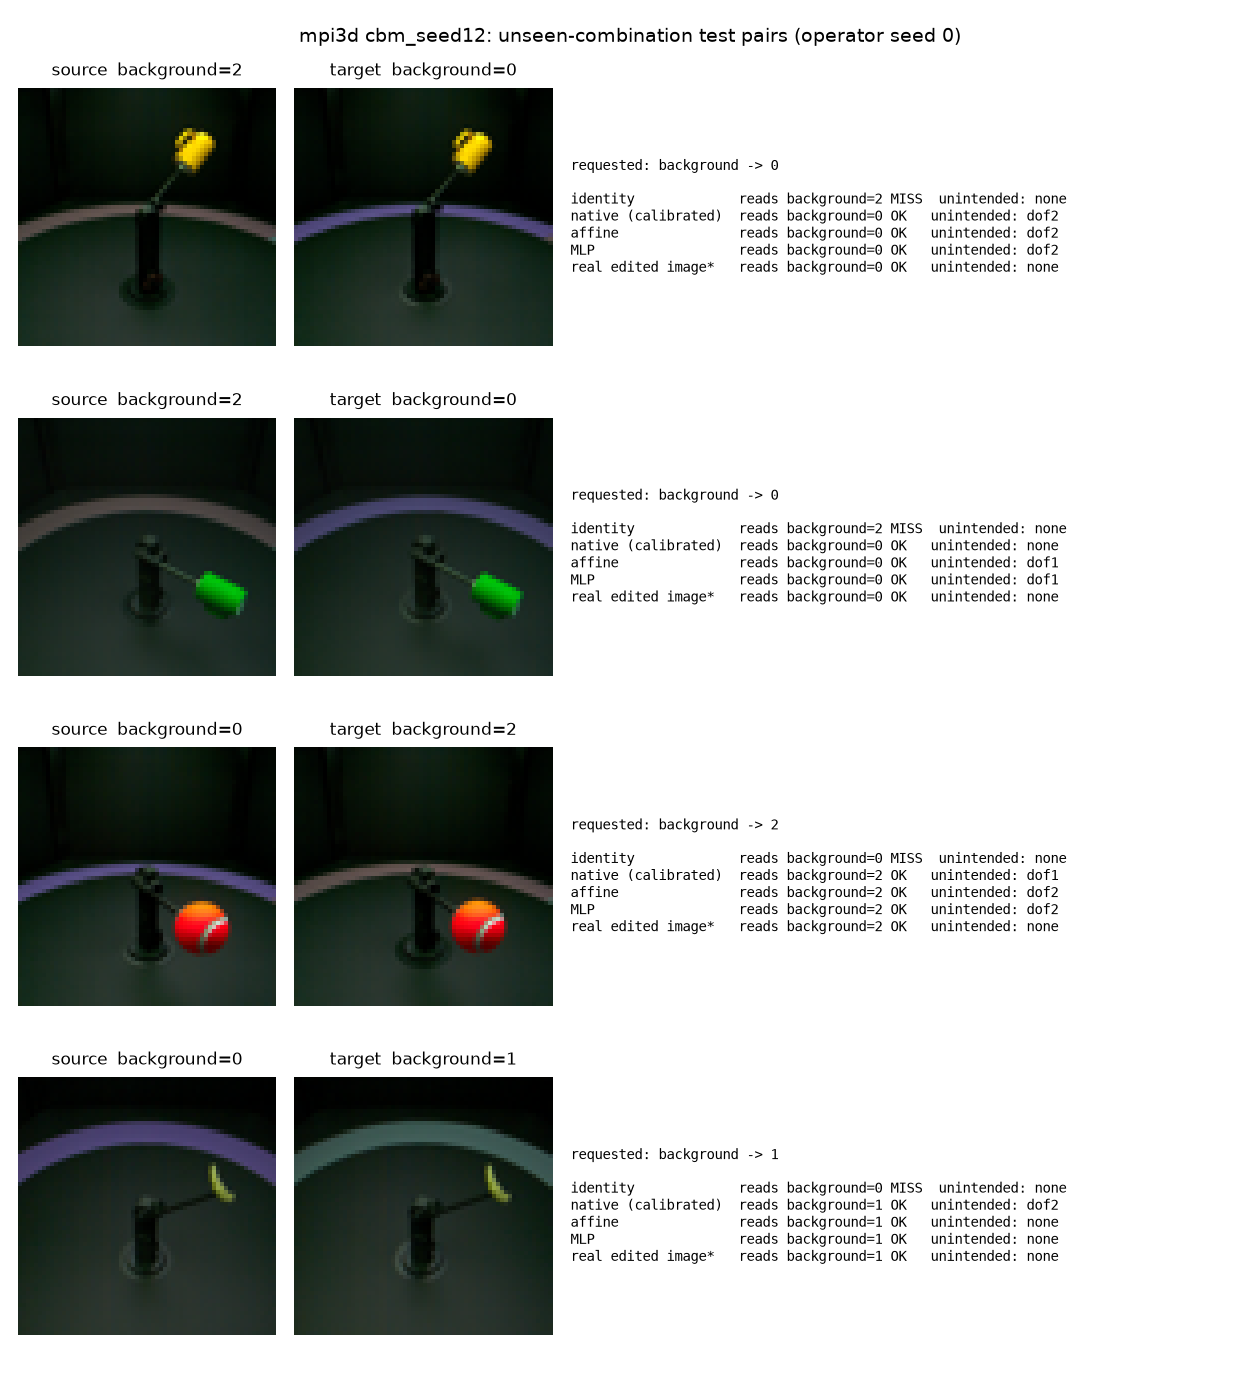
\includegraphics[width=0.92\textwidth]{figures/qualitative_mpi3d.png}
\caption{Qualitative examples, MPI3D CBM seed 12.}
\end{figure}

\end{document}
